% !TEX program = xelatex
\documentclass[11pt]{scrartcl}

% Compile with XeLaTeX (not pdflatex) -- required for Thai script shaping.
% e.g. `xelatex template.tex`, or `latexmk -xelatex template.tex`
\usepackage{fontspec}
\defaultfontfeatures{Mapping=tex-text}
% Main font is left unset, so English/Latin text keeps LaTeX's normal default
% (Latin Modern -- the standard Computer Modern look).

% TH Sarabun New is used ONLY for Thai text. Swap for e.g. "Leelawadee UI",
% "Angsana New", "Cordia New" if preferred.
\newfontfamily\thaifont{TH Sarabun New}[Scale=1.4]

% ucharclasses automatically switches to \thaifont whenever a character from
% the Thai Unicode block is encountered, and back to \normalfont as soon as
% the text leaves that block -- so English text and numbers stay in the
% default font with no manual markup needed.
\usepackage{ucharclasses}
\setTransitionsFor{Thai}{\thaifont}{\normalfont}

% Enables correct automatic line-breaking for Thai (no spaces between words),
% using XeTeX's built-in ICU line breaker. Does not affect English text.
\XeTeXlinebreaklocale "th_TH"
\XeTeXlinebreakskip = 0pt plus 1pt minus 1pt

\usepackage{amsmath,amssymb,amsthm,mathtools}

% Make \binom always render at display size (like \dbinom), even inline.
\renewcommand{\binom}[2]{\genfrac{(}{)}{0pt}{0}{#1}{#2}}

\usepackage[margin=1in]{geometry}
\usepackage{enumitem}
\usepackage{xcolor}
\usepackage[most]{tcolorbox}
\usepackage{tikz}
\usepackage{graphicx}
\graphicspath{{images/}}

\usepackage{multirow}
\usepackage{listings}
\usepackage{xcolor}

\lstset{
    language=Python,
    basicstyle=\ttfamily\small,
    keywordstyle=\color{blue},
    commentstyle=\color{gray},
    stringstyle=\color{red},
    frame=single,
    breaklines=true,
    showstringspaces=true
}

% Running head on every page: page number top-left, author name top-right.
\usepackage[headsepline]{scrlayer-scrpage}
\clearpairofpagestyles          % wipe KOMA's defaults (incl. the centred page number in the footer)
\lohead{\thepage}
\rohead{Anakawee Chujinda}
\pagestyle{scrheadings}
\renewcommand*{\pagemark}{\thepage}

\setlength{\parindent}{0pt}
\setlength{\parskip}{4pt}

\definecolor{probframe}{RGB}{30,30,30}
\definecolor{probback}{RGB}{246,246,246}
\definecolor{solframe}{RGB}{21,67,130}
\definecolor{solback}{RGB}{237,244,255}

\newtcolorbox{problembox}[1]{
  enhanced, breakable,
  colback=probback, colframe=probframe,
  boxrule=0.6pt, arc=1.5pt,
  top=3pt, bottom=3pt, left=7pt, right=7pt,
  fonttitle=\bfseries,
  coltitle=white, colbacktitle=probframe,
  title={#1}
}

\newtcolorbox{solutionbox}{
  enhanced, breakable,
  colback=solback, colframe=solframe,
  boxrule=0.6pt, arc=1.5pt,
  top=3pt, bottom=3pt, left=7pt, right=7pt,
  fonttitle=\bfseries,
  coltitle=white, colbacktitle=solframe,
  title={Solution}
}

\newlist{choices}{enumerate}{1}
\setlist[choices,1]{label=\arabic*), itemsep=1pt, topsep=3pt, leftmargin=2.4em}

\newlist{substmt}{enumerate}{1}
\setlist[substmt,1]{label=(\roman*), itemsep=1pt, topsep=3pt, leftmargin=2.6em}

\newcommand{\groupctx}[2]{\bigskip\noindent\textbf{Questions #1.} \textit{#2}\par\medskip}
\newcommand{\ans}[1]{\par\noindent\textbf{Answer: #1}\par}

\begin{document}

\begin{center}
{\LARGE\bfseries เฉลยคำตอบพร้อมวิธีทำ}\\[4pt]
{\large Midterm Exam วิชา 2110205 Statistics for Computer Engineering}\\[2pt]
{AUTHOR}
\end{center}

\bigskip
\hrule
\bigskip


\bigskip

% ---------------------------------------------------------------------------
% Shared context for a block of questions (optional):
% \groupctx{1--3}{Context text shared by problems 1 through 3.}
% ---------------------------------------------------------------------------

\begin{problembox}{Problem 1}
Which statement is correct about Bayesian's view of probability?

\begin{choices}
\item The probability of an event can be found by experimenting for a large amount of times.
\item The probability of an event can be different depending on the person.
\item Both are correct.
\item Both are incorrect.
\end{choices}
\end{problembox}

\begin{solutionbox}
  มุมมองความน่าจะเป็นของ Bayesian เป็นการมองโจทย์ปัญหาทางหลักการนับและสถิติโดยยึดความเชื่อมั่นจากความรู้และสิ่งที่เชื่อ
  
  มุมมองของ Frequentist เป็นการมองโจทย์ปัญหาทางหลักการนับและสถิติโดยยึดจากการทดลองและสังเกตการณ์เป็นจำนวนมาก
  
  สำหรับข้อนี้จึงควรเลือกตอบข้อที่ 2) เพราะเป็นการหาความน่าจะเป็นจากสิ่งที่ขึ้นอยู่กับแต่ละคน

  ตอบ $\boxed{2)}$
\end{solutionbox}

\begin{problembox}{Problem 2}
Which student is applying statistical analysis?

\begin{choices}
\item Somnuke picks the horse that is most likely to win by using data from the past 3 years.
\item Pawit assumes each horse having equal chance of winning. Then, he writes a computer program that will determine the best betting strategy via simulation.
\item Alan always pick the horse which is his lucky number.
\item Bart uses a 10-sided die to determine the horse to bet on.
\end{choices}
\end{problembox}

\begin{solutionbox}
  Statistical Analysis คือการวิเคราะห์ทางสถิติซึ่งต้องอาศัยผลการทดลอง/สังเกต/การบันทึกของที่ผ่านมาเพื่อวิเคราะห์ข้อมูลเพิ่มเติมให้นำมาซึ่งคำตอบ ซึ่งตรงกับข้อที่ 1)
  เนื่องจากข้ออื่นเป็นการใช้ข้อมูลที่ไม่จำเป็นต้องเก็บข้อมูลเพิ่มเติมเพื่อหาคำตอบและยังมีความน่าจะเป็นที่เท่ากันในทุกเหตุการณ์อย่างแน่นอน

  ตอบ $\boxed{1)}$
\end{solutionbox}

\newpage

\begin{problembox}{Problem 3}
In pandas, what does the function .unique() do?

\begin{choices}
\item Returns a random unique value for every row.
\item Remove all non-unique values in a dataframe.
\item Return a list of unique values in a column.
\item Sorts the dataframe using the unique values.
\end{choices}
\end{problembox}

\begin{solutionbox}
  ตอบ $\boxed{3)}$
\end{solutionbox}

\begin{problembox}{Problem 4}
Given a dataframe

\begin{center}
\begin{tabular}{lccc}
        & & Type & Speed \\
\multirow{2}{*}{Falcon} & & 0 & 200 \\
        & & 1 & 240 \\
\multirow{2}{*}{Parrot} & & 0 & 100 \\
        & & 1 & 110 \\
\end{tabular}
\end{center}

If we apply the command, \texttt{df.groupby("Type").mean()} what would be the output?

\begin{center}
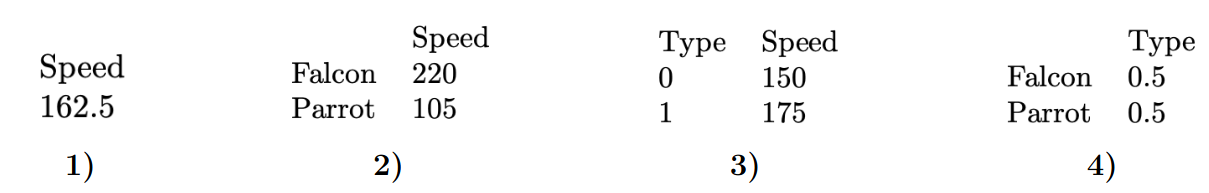
\includegraphics[width=0.8\textwidth]{q4_df-type_statement.png}
\end{center}

\end{problembox}

\begin{solutionbox}
  การทำงานของคำสั่ง \texttt{.groupby("Type")} จะเป็นการนำทุกค่าที่อยู่ใน \texttt{"Type"} เดียวกันมา Aggregation (การรวมกลุ่ม) โดยการหาค่า Mean ทำให้สามารถคำนวณออกมาได้ดังนี้:

  \begin{align*}
    \text{Type}_0 &= \frac{200+100}{2} = 150 \\
    \text{Type}_1 &= \frac{240+110}{2} = 175
  \end{align*}
  ตอบ $\boxed{3)}$
\end{solutionbox}

\newpage

\begin{problembox}{Problem 5}
According to the following code, what is the probability that the speed is 100?

\begin{lstlisting}
import random
speed = 50
if random.randint(0,2): # uniform discrete from 0 to 2
    speed = speed*2
if random.random() > 1: # uniform continuous from 0 to 1
    speed = speed*2
print(speed)
\end{lstlisting}

\begin{choices}
\item 25\%
\item 33\%
\item 50\%
\item 67\%
\end{choices}
\end{problembox}

\begin{solutionbox}
  เมื่อเราอ่าน Code ที่ปรากฏข้างต้นเราจะทราบว่าใน If-block แรกจะมีเพียงแค่เหตุการณ์ที่สุ่มออกมาแล้วทำให้ \texttt{speed = 100} นั้นมีเพียง 2 เหตุการณ์จากทั้งหมด 3 นั่นคือ 1, 2
  จึงทำให้ทราบได้ว่าความน่าจะเป็นที่จะเกิดเหตุการณ์ดังกล่าวคือ $\frac{2}{3} \approx 0.66\overline{6} \approx 67\%$

  ตอบ $\boxed{4)}$
\end{solutionbox}

\begin{problembox}{Problem 6}
100 students were asked to fill the following survey. 40\% answer “C++”, 20\% answer “Java”, and 10\% answer “Both”. How many students can code in at least one language?

\textbf{Survey:} \textit{Which language can you code in? (Choose one answer.)}


\vspace{3pt}
$\square$ C++ \hfill $\square$ Java \hfill $\square$ Both \hfill $\square$ Neither

\begin{choices}
\item 30
\item 50
\item 70
\item 90
\end{choices}
\end{problembox}

\begin{solutionbox}
  \underline{\textbf{Solution-1}}

  โจทย์ข้อนี้ได้มีการระบุข้อจำกัดในแบบสำรวจแล้วว่าคน ๆ หนึ่งเลือกตอบได้เพียง 1 คำตอบเท่านั้น 
  นั่นทำให้เราเก็บข้อมูลแยกรายตัวเลือกได้ทันทีโดยไม่ต้องทำการคำนวณเลย ทำให้คำนวณได้โดยตรงคือนำจำนวนยอดที่กรอกแต่ละแบบมาบวกได้โดยตรง
  คิดได้จาก $40+20+10 = 70$ คน

  \underline{\textbf{Solution-2}}
  \begin{flushleft}
  $\begin{aligned}
    \text{กำหนดให้ } A &:= \text{คนที่เขียนภาษา C++ ได้} \\
    B &:= \text{คนที่เขียนภาษา Java ได้}
  \end{aligned}$
  \end{flushleft}

  จากสิ่งที่กำหนดทำให้ทราบเพิ่มเติมว่า $n(A-B) = 40, n(B-A) = 20, n(A \cap B) = 10$ 
  โจทย์ต้องการทราบว่า $n(A \cup B)$ มีค่าเท่าใด ทำให้สามารถคิดโดยนำมาบวกได้โดยตรง คิดจาก $40+20+10 = 70$ คน
  
  ตอบ $\boxed{3)}$
\end{solutionbox}

\begin{problembox}{Problem 7}
Consider the following Python code.
\begin{lstlisting}
s=1
for i in range(1,n):
  s=s*i
for i in range(1,k):
  s=s/i
print(s)
\end{lstlisting}
What does this code compute?
\begin{choices}
\item $_n P_k$
\item $_{n-1} P_{k-1}$
\item $_n P_{n-k}$
\item $_{n-1} P_{n-k}$
\end{choices}
\end{problembox}

\begin{solutionbox}
  ทำการวิเคราะห์ว่าจาก Python Code ที่ระบุข้างต้นทำงานได้อย่างไร โดยเริ่มต้นจาก...
  \begin{itemize}
    \item For-block แรกทำงานตั้งแต่ $[1, n-1]$ ทำให้เรามีค่าตัว $s$ อยู่ที่ $1 \times 2 \times ... \times (n-1) = (n-1)!$
    \item For-block สองทำงานตั้งแต่ $[1, k-1]$ ทำให้เรามีค่าตัว $s$ อยู่ที่ $1 \times 2 \times ... \times (k-1) = (k-1)!$
    \item เมื่อเขียนเป็นรูปสมการคณิตจะได้ว่า $\frac{1 \times 2 \times ... \times (n-1)}{1 \times 2 \times ... \times (k-1)} = \frac{(n-1)!}{(k-1)!}$
  \end{itemize}
  เพื่อความง่ายตรวจสอบ ให้ลองทำการแทนค่าสำหรับตัวแปร $n, k$ มีค่าห่างที่ห่างกัน ณ ที่นี้ขอสมมติค่าเป็น $n=8, k=5$ จากรูปสมการเศษส่วนด้านบนจึงได้ว่า $\frac{7!}{4!}$ ถัดไปทำการหาว่าตัวเลือกในข้อสอบใดมีค่าตรงกับเศษส่วนข้างต้น ซึ่งแทนที่ตัวเลขได้ดังนี้...
  \begin{itemize}
    \item ${}_nP_k = {}_8P_5 = \frac{8!}{3!}$
    \item ${}_{n-1}P_{k-1} = {}_7P_4 = \frac{7!}{3!}$
    \item ${}_nP_{n-k} = {}_8P_3 = \frac{8!}{5!}$
    \item ${}_{n-1}P_{n-k} = {}_7P_3 = \frac{7!}{4!}$
  \end{itemize}

  ตอบ $\boxed{4)}$
\end{solutionbox}

\newpage

\begin{problembox}{Problem 8}
In September, 18 days are sunny, 14 days are rainy, and 5 days are neither sunny nor rainy. How many days in September are both sunny and rainy?

\begin{choices}
\item 3
\item 5
\item 7
\item 9
\end{choices}
\end{problembox}

\begin{solutionbox}
  \begin{flushleft}
  $\begin{aligned}
    \text{กำหนดให้ } n(A) &:= \text{จำนวนวันที่แดดจ้า} \\
    n(B) &:= \text{จำนวนวันที่ฝนตก}
  \end{aligned}$
  \end{flushleft}

  โดยโจทย์ระบุข้อมูลแต่ละส่วนดังนี้ $n(A) = 18, n(B) = 14, n((A \cup B)') = 5$ โจทย์ต้องการหา $n(A \cap B)$ สามารถหาได้โดยใช้หลักการ Inclusion-Exclusion Principle นั่นคือ 
  \begin{align*}
    n(A \cup B) = n(A)+n(B)-n(A \cap B)
  \end{align*}

  จากข้อมูลที่มีในปัจจุบันเมื่อทำการวาด Venn Diagram จะได้ว่า

  \begin{center}
  \begin{tikzpicture}
      % Universal set
      \draw (-4,-3) rectangle (4,3);
      \node at (-2.95,2.5) {$U=30$};

      % Set A background
      \fill[blue!20] (-1.2,0) circle (2);

      % Set B background
      \fill[red!20] (1.2,0) circle (2);

      % A ∩ B background
      \begin{scope}
          \clip (-1.2,0) circle (2);
          \fill[purple!40] (1.2,0) circle (2);
      \end{scope}

      % Set A border
      \draw (-1.2,0) circle (2);

      % Set B border
      \draw (1.2,0) circle (2);

      % Labels
      \node at (-1.5,1.5) {$A$};
      \node at (1.5,1.5) {$B$};

      % Elements in each region
      \node at (-2.0,0) {$18-x$};
      \node at (0,0) {$x$};
      \node at (2.0,0) {$14-x$};
      \node at (3.2,-2.2) {$5$};

  \end{tikzpicture}
  \end{center}

  จากการที่เราทราบค่าของ $n((A \cup B)')$ จึงทำให้ทราบค่า $n(A \cup B) = n(U) - n((A \cup B)') = 30-5 = 25$ จึงทำให้เราหา $n(A \cap B)$ ได้โดยคำนวณดังต่อไปนี้
  \begin{align*}
    n(A \cup B ) &= n(A)+n(B)-n(A \cap B) \\
        25       &=  18+14-n(A \cap B) \\
    n(A \cap B)  &=  32-25 \\
    n(A \cap B)  &=  7 \\
  \end{align*}
  ตอบ $\boxed{3)}$
\end{solutionbox}

\begin{problembox}{Problem 9}
How many integers from 1 to 1,000 are divisible by 4 but not divisible by 5?
 
\begin{choices}
\item 150
\item 200
\item 230
\item 400
\end{choices}
\end{problembox}

\begin{solutionbox}
  \begin{flushleft}
  $\begin{aligned}
    \text{กำหนดให้ } n(A) &:= \text{จำนวนตัวเลขที่หาร 4 ลงตัว} \\
    n(B) &:= \text{จำนวนตัวเลขที่หาร 5 ลงตัว}
  \end{aligned}$
  \end{flushleft}

  จากที่โจทย์ระบุ ทำให้ได้ข้อมูลแต่ละส่วนดังนี้ $n(A) = \frac{1000}{4} = 250, n(B) = \frac{1000}{5} = 200, n(A \cap B) = \frac{1000}{gcd(4, 5)} = 50$ โจทย์ต้องการหา $n(A \cap B')$ สามารถหาได้โดย...
  \begin{align*}
    n(A \cap B') &= n(A) - n(A \cap B) \\
                  &= 250 - 50 \\
                  &= 200 \\
  \end{align*}
  สาเหตุที่สามารถหาโดยใช้ $n(A) - n(A \cap B)$ ได้นั่นเพราะความหมายของ $n(A \cap B')$ คือเอาของที่มีใน A แต่ไม่มีใน B ซึ่งหากลองวาดภาพ Venn Diagram ก็จะพบว่าสามารถคำนวณได้ด้วยวิธีข้างต้น

  \begin{center}
  \begin{tikzpicture}
      % Universal set
      \draw (-4,-3) rectangle (4,3);
      \node at (-2.95,2.5) {$U=1000$};

      % Set A background
      \fill[blue!20] (-1.2,0) circle (2);

      % Set B background
      % \fill[red!20] (1.2,0) circle (2);

      % A ∩ B background
      \begin{scope}
          \clip (-1.2,0) circle (2);
          \fill[purple!40] (1.2,0) circle (2);
      \end{scope}

      % Set A border
      \draw (-1.2,0) circle (2);

      % Set B border
      \draw (1.2,0) circle (2);

      % Labels
      \node at (-1.5,1.5) {$A$};
      \node at (1.5,1.5) {$B$};

      % Elements in each region
      \node at (-2.0,0) {$250-50$};
      \node at (0,0) {$50$};
      \node at (2.0,0) {$200-50$};

  \end{tikzpicture}
  \end{center}

  ตอบ $\boxed{2)}$
\end{solutionbox}

\newpage

\begin{problembox}{Problem 10}
There are 5 men and 3 women in the CEDT student council. They want to select a president, first vice president, second vice president, and secretary. The first vice president must be a woman and the second vice president must be a man, while the president and secretary can be any gender. How many ways can they select the positions if each person can hold at most one position?
 
\begin{choices}
\item 360
\item 390
\item 420
\item 450
\end{choices}
\end{problembox}

\begin{solutionbox}
  จากโจทย์ระบุว่า
  \begin{itemize}
    \item มีผู้ชาย 5 คน และผู้หญิง 3 คน
    \item ต้องการเลือกตำแหน่งโดยที่แต่ละคนมีได้มากสุด 1 ตำแหน่ง
    \item First vice president ต้องเป็นผู้หญิง และ Second vice president ต้องเป็นผู้ชาย 
  \end{itemize}
  
  ทำการหยิบเลือกบุคคลที่มีข้อจำกัดมากที่สุดก่อนนั่นคือ First/Second vice president และอีก 2 ตำแหน่งที่เหลือไม่ระบุเงื่อนไขแต่สามารถมีได้เพียงแค่คนเดียว ทำให้คำนวณได้ว่า $3 \times 5 \times 6 \times 5 = 450$ วิธี

  ตอบ $\boxed{4)}$
\end{solutionbox}
 
\begin{problembox}{Problem 11}
There are 5 men and 5 women in a class. They want to select 4 students to attend a conference, which must consist of at least one man and at least one woman. How many ways can they select students to attend the conference?
 
\begin{choices}
\item 140
\item 200
\item 210
\item 700
\end{choices}
\end{problembox}

\begin{solutionbox}
  จากโจทย์ระบุว่า
  \begin{itemize}
    \item มีผู้ชาย 5 คน และผู้หญิง 5 คน
    \item มีคนต้องถูกเลือกไปประชุมทั้งสิ้น 4 คน
    \item ต้องการเลือกผู้ชายและผู้หญิงพร้อมกันอย่างน้อย 1 คนไปประชุม จัดได้กี่วิธี
  \end{itemize}
  ใช้หลักการลบแบบ Complement ซึ่งมีหลักดังต่อไปนี้
  \begin{align*}
    n(\text{กรณีที่สนใจ}) &= n(\text{วิธีจัดกรณีไม่มีข้อจำกัด}) - \sum_{k=1}^{n(\text{กรณีที่ผิด})} n(\text{กรณีที่ผิด}_k)
  \end{align*}

  ในที่นี้มีกรณีที่ผิดกฏอยู่ 2 แบบคือเลือกเพียงผู้ชายเท่านั้นกับเลือกเพียงผู้หญิงเท่านั้นซึ่งสามารถคำนวณได้ดังนี้

  \begin{align*}
    \text{กรณีเลือกโดยไม่มีข้อจำกัด} &= \binom{10}{4} = 210 \text{ วิธี} \\
    \text{กรณีเลือกแต่ผู้ชาย} &= \binom{5}{4} = 5 \text{ วิธี} \\
    \text{กรณีเลือกแต่ผู้หญิง} &= \binom{5}{4} = 5 \text{ วิธี} \\
  \end{align*}

  $\therefore n(\text{กรณีที่สนใจ}) = 210 - 5 - 5 = 200 \text{ วิธี}$

  ตอบ $\boxed{2)}$
\end{solutionbox}

\begin{problembox}{Problem 13}
The CU equestrian club has 12 members. 3 of them are first-year students, 4 are second-year students, and 5 are third-year students. If we randomly select 3 club members, what is the probability that they are all in the same year?
 
\begin{choices}
\item $1/10$
\item $1/20$
\item $3/11$
\item $3/44$
\end{choices}
\end{problembox}

\begin{solutionbox}
  จากโจทย์ระบุว่า
  \begin{itemize}
    \item ชมรมมีสมาชิกทั้งสิ้น 12 คน
    \item เป็นนักเรียนปี 1 จำนวน 3 คน
    \item เป็นนักเรียนปี 2 จำนวน 4 คน
    \item เป็นนักเรียนปี 3 จำนวน 5 คน
    \item หาความน่าจะเป็นของต้องการเลือก 3 คนและมีแต่ปีเดียวกัน
  \end{itemize}
  
  ทำให้เราสามารถหาค่า $n(S) = \binom{12}{3} = 220$ และเราสามารถหาค่าของ $n(E)$ ได้โดยการรวมทุกกรณีย่อย ซึ่งสามารถคิดแต่ละกรณีย่อยได้ดังนี้...
  \begin{align*}
    \text{เลือกเพียงปี 1} &= \binom{3}{3} = 1 \text{ วิธี} \\
    \text{เลือกเพียงปี 2} &= \binom{4}{3} = 4 \text{ วิธี} \\
    \text{เลือกเพียงปี 3} &= \binom{5}{3} = 10 \text{ วิธี} \\
  \end{align*} 
  จึงรวมค่า $n(E) = 1+4+10 = 15$
  $\therefore$ ความน่าจะเป็นจึงมีค่า = $\frac{15}{220} = \frac{3}{44}$

  ตอบ $\boxed{4)}$
\end{solutionbox}

\begin{problembox}{Problem 14}
4 players are playing Among Us. Each player can vote for one other player (but cannot vote for him/herself). If every player votes randomly, what is the probability that there is a player who receives exactly 3 votes.
 
\begin{choices}
\item $1/81$
\item $1/27$
\item $4/27$
\item $4/81$
\end{choices}
\end{problembox}

\begin{solutionbox}
  จากโจทย์ระบุว่า
  \begin{itemize}
    \item มีผู้เล่นในเกม Among Us ทั้งสิ้น 4 คน
    \item แต่ละคนโหวตได้เพียงแค่ 1 คนเท่านั้น (โหวตตัวเองไม่ได้)
    \item หาความน่าจะเป็นที่ผู้เล่นคนหนึ่งถูกโหวต 3 ครั้งพอดี
  \end{itemize}

  จากข้อมูลที่ได้รับทำให้ทราบว่า $n(S) = 3^4 = 81$ การหาค่า $n(E)$ สามารถหาได้จากการนับจำนวน\textbf{วิธีการถูกโหวต}ของผู้เล่นหมายเลขนั้น ๆ ซึ่งคำนวณได้จาก
  \begin{align*}
    n(\text{โหวตแต่ผู้เล่น No.1}) &= 3 \text{ (ผู้เล่นคนที่ 1 เลือกได้)} \times 1 \text{ (ผู้เล่นที่เหลือเลือกได้)} = 3 \\
    &\vdots \\
    n(\text{โหวตแต่ผู้เล่น No.4}) &= 3 \text{ (ผู้เล่นคนที่ 4 เลือกได้)} \times 1 \text{ (ผู้เล่นที่เหลือเลือกได้)} = 3
  \end{align*}

  นำกรณีที่โหวตแต่ละผู้เล่นมารวมกันจะได้ $3 \times 4 \text{ (จำนวนผู้เล่นทั้งหมด)} = 12$ 
  
  $\therefore$ ความน่าจะเป็นจึงมีค่า $\frac{12}{81} = \frac{4}{27}$

  ตอบ $\boxed{3)}$
\end{solutionbox}

\groupctx{29--30}{Students in a particular university are either in the CEDT or CP program. 60\% of CEDT students and 30\% of CP students can write JavaScript. Overall, 48\% of students in this university can write JavaScript.}
 
\begin{problembox}{Problem 29}
If a student can write JavaScript, what is the probability that this student is in CEDT program?
 
\begin{choices}
\item $3/4$
\item $4/5$
\item $5/6$
\item $6/7$
\end{choices}
\end{problembox}

\begin{solutionbox}
  \begin{flushleft}
  $\begin{aligned}
    \text{กำหนดให้ } A &:= \text{นิสิต CEDT} \\
    B &:= \text{นิสิต CP} \\
    J &:= \text{เขียน JavaScript ได้} \\
  \end{aligned}$
  \end{flushleft}

  จากโจทย์ระบุว่า $P(J) = 0.48, P(J|A) = 0.6, P(J|B) = 0.3$ สำหรับข้อนี้โจทย์ต้องการหา $P(A|J)$

  ใช้ทฤษฎีบทของ Bayes Theorem ในการหาค่าความน่าจะเป็นย้อนกลับจาก ซึ่งได้ว่า $P(A|J) = \frac{P(J|A)P(A)}{P(J)}$ แต่ตอนนี้เรายังไม่ทราบค่าของ $P(A)$ จึงยังทำให้หาค่าไม่ได้
  สำหรับโจทย์ข้อนี้วิธีหา $P(A)$ ที่ง่ายที่สุดคือหาจาก $P(J)$ โดยใช้หลักการของ Law of Total Probability ทำให้สามารถคำนวณออกมาได้ดังนี้
  \begin{align*}
    P(J) &= P(J|A)P(A) + P(J|B)P(B) \\
    0.48  &= 0.6x + 0.3(1-x) \\
    0.48  &= 0.6x + 0.3 - 0.3x \\
    0.3x  &= 0.18 \\
    x  &= \frac{0.18}{0.3} = 0.6 \\
  \end{align*}

  โดยจากการแก้สมการข้างต้นนั้นได้แทนที่ $x = P(A)$ และ $P(B) = 1-x$ เพราะ $P(B)$ สามารถหาได้โดยการนำจำนวนยอดร้อยละทั้งหมดมาหักหับยอดความน่าจะเป็นของการเกิด $P(A)$ เมื่อรู้เช่นนั้นแล้วจึงแก้สมการออกมาและได้ผลลัพธ์ $P(A) = 0.6$ 

  เมื่อได้ค่า $P(A)$ แล้วจึงนำกลับมาแทนค่าในสมการของ Bayes Theorem ต่อดังนี้
  \begin{align*}
    P(A|J) &= \frac{P(J|A)P(A)}{P(J)} \\
          &= \frac{0.6 \times 0.6}{0.48} \\
          &= 0.75 \; \left(\text{หรือ } \frac{3}{4}\right)
  \end{align*}

  ตอบ $\boxed{1)}$
\end{solutionbox}
 
\begin{problembox}{Problem 30}
If a student cannot write JavaScript, what is the probability that this student is in CEDT program?
 
\begin{choices}
\item $3/13$
\item $4/13$
\item $5/13$
\item $6/13$
\end{choices}
\end{problembox}

\begin{solutionbox}
  โจทย์ข้อนี้ต้องการทราบ $P(A|J')$ ซึ่งสามารถคิดได้จาก Bayes Theorem ดังนี้
  \begin{align*}
    P(A|J') &= \frac{P(J'|A)P(A)}{P(J')} \\
          &= \frac{0.4 \times 0.6}{0.52} \\
          &\approx 0.46153 \; \left(\text{หรือ } \frac{6}{13}\right)
  \end{align*}
  
  ตอบ $\boxed{4)}$

  \underline{\textbf{Notes:}}
  เราสามารถหาค่าของ $P(J'|A)$ ได้หากทราบค่า $P(J|A)$ โดยการนำ $1 - P(J|A) = 1-0.6 = 0.4$
\end{solutionbox}

\begin{problembox}{Problem 1}
Problem statement here.

% Optional (i)/(ii)/(iii) sub-statements:
% \begin{substmt}
% \item First statement.
% \item Second statement.
% \end{substmt}

\begin{choices}
\item Choice one
\item Choice two
\item Choice three
\item Choice four
\end{choices}
\end{problembox}

\begin{solutionbox}
  Solution text here (Thai or English).
  \begin{align*}
    a &= b \\
      &= c
  \end{align*}
  ตอบ $\boxed{1)}$
\end{solutionbox}


\end{document}